%%%%%%%%%%%%%%%%%%%%%%%%%%%%%%%%%%%%%%%%%%%%%%%%%%%%%%%%%%%%%%%%%%%%%%%%
%                                                                      %
%     File: Thesis_Exploratory_Ideas.tex                                      %
%     Tex Master: Thesis.tex                                           %
%                                                                      %
%     Author: Andre C. Marta                                           %
%     Last modified :  4 Mar 2024                                      %
%                                                                      %
%%%%%%%%%%%%%%%%%%%%%%%%%%%%%%%%%%%%%%%%%%%%%%%%%%%%%%%%%%%%%%%%%%%%%%%%

\chapter{Alternative Schemes}
\label{chapter:Exploratory_Ideas}

In this chapter, we will present alternative schemes that, although not entirely based on the \acrshort{iqaqe} Framework, emerged from our research on these topics. These are different algorithms proposed to solve the \acrshort{maxcut} problem.

%%%%%%%%%%%%%%%%%%%%%%%%%%%%%%%%%%%%%%%%%%%%%%%%%%%%%%%%%%%%%%%%%%%%%%%%
\section{Parity-like QAOA}
\label{section:Parity_QAOA}

The next idea we will explore involves "reducing" \acrshort{qaoa}'s problem Hamiltonian to use fewer qubits than usual. To achieve this, we will utilize parity encodings, which allow us to compress the representation of \(N\) nodes into \(n < N\) qubits (with \(N = \mathcal{O}(n^k)\), for any \(k\)\footnote{This $k$ is equivalent to the previously mentioned $k$ in polynomial compression-based schemes.}, as long as \(\binom{n}{k} \geq N\)). In this scheme, \acrshort{qaoa}'s problem Hamiltonian, the usual
\begin{equation}\label{eq:H_P-QAOA}
    H_P = \frac{1}{2}\sum\limits_{i<j}(1-Z_iZ_j),
\end{equation}
gets "unfolded" into:
\begin{equation}\label{eq:H_P-QAOA-k=2}
    H_P = \frac{1}{2}\sum\limits_{i \leq k<l;i<j \leq l}(1-Z_iZ_jZ_kZ_l),
\end{equation}
for example, when performing quadratic compression with \(k = 2\). (The sums are taken over the graph's edges, as is customary.) Each node is now associated with a tuple of \(k = 2\) qubits, and the node's set/color is determined by the parity of those \(k\) qubits (Even number of $1$'s: Set $0$; Odd number of $1$'s: Set $1$). This criterion is used to obtain the final partition, after training, from the most frequently sampled bit-string. The terms with $4$ Pauli-$z$ operators (when \(k = 2\)) can be understood as a product of two terms with $2$ Pauli-$z$ operators. Each of these terms represents the set/color of the corresponding nodes for each edge in the graph. It is easy to verify that this product gives $-1$ when the individual nodes belong to different sets, as expected. Additionally, note that any value of \(k\) can be used, as long as we can encode all necessary nodes in that many qubits (Number of possible encodings \(= \binom{n}{k} \implies N = \mathcal{O}(n^k)\)). Then, \(n\) is taken as the smallest value that satisfies \(\binom{n}{k} \geq N\), similar to the previous polynomial compression-based algorithm. Furthermore, this approach can be generalized to other values of \(k\) by "unfolding" each \(Z_i\) in the \(Z_i Z_j\) terms of Eq. \ref{eq:H_P-QAOA} into products of \(k\) Pauli-$z$'s, according to the specified encoding. A minimal example is provided below. This was kindly produced by Bence Bakó. This example aims to give more intuition on how this method works in practice.

% Re-write from here onwards.
Suppose we are solving \acrshort{maxcut} on a $6$-node graph using this Parity-like \acrshort{qaoa} with $k=2$, resulting in a problem Hamiltonian similar to the one described in Eq. \ref{eq:H_P-QAOA-k=2}. This is achieved by compressing the usual $6$-qubit representation (\acrshort{qaoa}) to use only $4$ qubits (\(\binom{4}{2} = 6 \geq 6\)) with the following mapping:
\begin{center}
\begin{adjustwidth}{2.5cm}{0cm}
\begin{multicols}{2}
\begin{itemize}
    \item Node $0 \rightarrow$ Qubits $(0,1),$
    \item Node $1 \rightarrow$ Qubits $(0,2),$
    \item Node $2 \rightarrow$ Qubits $(0,3),$
    \item Node $3 \rightarrow$ Qubits $(1,2),$
    \item Node $4 \rightarrow$ Qubits $(1,3),$
    \item Node $5 \rightarrow$ Qubits $(2,3).$
\end{itemize}
\end{multicols}
\end{adjustwidth}
\end{center}
With this problem Hamiltonian, the standard QAOA ansatz – adapted to the scheme – can be implemented using the expectation value as the cost function. The corresponding $4$-qubit operators \( e^{-i\alpha Z_iZ_jZ_kZ_l/2} \) can be implemented as illustrated in Figure \ref{fig:decomposition}.
\begin{figure}[H]
\centering
\begin{quantikz}
\lstick{Qubit i} & \ctrl{1} & \qw  & \qw & \qw & \qw & \qw & \ctrl{1} & \qw & \\
\lstick{Qubit j} & \targ{} & \ctrl{1} & \qw & \qw & \qw  & \ctrl{1} & \targ{} & \qw & \\
\lstick{Qubit k} & \qw & \targ{} & \ctrl{1} & \qw & \ctrl{1} & \targ{} & \qw & \qw & \\
\lstick{Qubit l} & \qw & \qw & \targ{} & \gate{R_z(\alpha)} & \targ{} & \qw & \qw & \qw & \\
\end{quantikz}
\caption{$e^{-i\alpha Z_i Z_j Z_k Z_l/2}$ decomposition.\label{fig:decomposition}}
\end{figure}
With this approach, we effectively reduced the number of qubits from $6$ to $4$, but at the cost of a deeper circuit. The mapping is flexible and does not have to be to an equal number of qubits; one can mix mappings to $1$, $2$, $3$, or any number of qubits. The encoding aspect of this idea is essentially the same as in \cite{sciorilli2024largescale}, restricted to the $Z$ basis. This can also be seen as a type of parity encoding, since we multiply Pauli-$z$ matrices, which have eigenvalues of $\pm 1$. This also shares some similarity with \cite{ender2022modular}.

% Re-read from here onwards: most likely, I'll have to cut some things out.
Now, I present the outcomes of the numerical simulation of Parity-like \acrshort{qaoa} for the \acrshort{maxcut} problem on the standard $8$-node graph. These results are depicted in Figure \ref{fig:parity_qaoa_results}.
\begin{figure}[t]
    \centering
    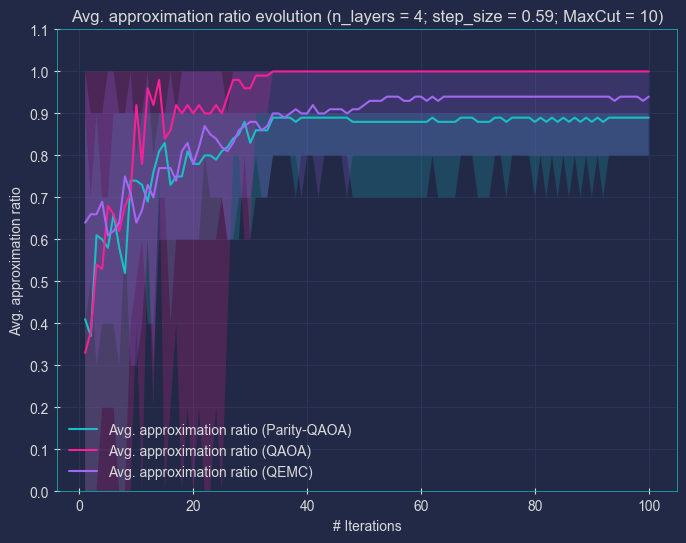
\includegraphics[width=1\textwidth]{Figures/Chapter_6/Parity_QAOA.png}
    \caption{Results from the numerical simulation of Parity-like \acrshort{qaoa} ($k=2$) applied to the \acrshort{maxcut} problem on the standard $8$-node graph.}
    \label{fig:parity_qaoa_results}
\end{figure}
It became apparent that, for $k = 2$, the specified encoding appeared incapable of generating the \acrshort{maxcut} partition (cf. Figure \ref{fig:parity_qaoa_results}). This sparked discussions regarding the generality of such an encoding. If the \acrshort{maxcut} partition cannot be constructed using this encoding, then achieving it through our ansatz becomes unattainable. This constitutes a significant flaw. Further insights arose from discussions with Prof. Zoltán Zimboras and others, emphasizing the presence of "cycles" in our encoding. These cycles impede our ability to encode all desired states, effectively tying certain nodes to the parity of others and automatically excluding certain partitions from our operational domain. Initially, the goal was to completely avoid such cycles. However, it has become clear that completely eliminating them is impossible. These cycles emerge as a result of confining the problem to a reduced subspace.

For instance, in a $6$-node graph encoded in $4$ qubits, there are $2$ cycles: $0, 1, 3$ and $3, 4, 5$ (from the previous example encoding). The occurrence of these cycles is not incidental; reducing from $6$ qubits to $4$ imposes two constraints, represented by these cycles. Hence, it is theoretically impossible to encode all potential $6$-node partitions in the given $4$ qubits. Unless the encoding ensures the inclusion of the \acrshort{maxcut} partition within this reduced space, the scheme appears destined to fail in theory. Achieving such a feat would be remarkable, though, as it would effectively diminish the problem size, thereby enhancing the search process. However, I am uncertain about its feasibility. Mastering this encoding would likely necessitate specific graph instance knowledge. Given the variability in graph instances, devising a universal rule seems improbable.

Additionally, it was observed that the symmetry property, previously confirmed for standard \acrshort{qaoa}\footnote{Wherein original and inverted bit-strings, e.g., $1001$ and $0110$, represent identical partitions (though with different labels) and are thus trained to achieve identical probabilities.}, was only upheld when $k$ was odd. In cases where $k$ was even, inverting the bit-string produced the exact same partition, indicating that one possible \acrshort{maxcut} partition was overlooked by the algorithm.

Furthermore, while implementing the algorithm, it was found that despite the encoding leading to deeper Ansätze, the outcomes were not as dire as initially anticipated. This was due to the simplification of terms such as $e^{Z_0Z_1Z_0Z_2}$ to $e^{Z_1Z_2}$, resulting in simpler circuits compared to those for $4$ Pauli-$z$'s (which could be more than $4$ depending on the value of $k$). It was also confirmed that the ordering of terms in the complex exponential was irrelevant, allowing for flexibility in reordering terms to streamline implementation.

% Here, onwards, I'll have to re-write everything.
Inspired by \cite{sciorilli2024largescale}, an effort was made to address the encoding issue stemming from the previously identified "cycles". These cycles were interpreted as manifestations of frustration effects, akin to those observed in antiferromagnetic spin chains. To mitigate these effects, a regularization term was introduced into the problem Hamiltonian. This term coerces the expectation values, necessary for computing the cost function, to approach zero, thereby reducing the impact of frustration. This approach entails modifying the read-out process to ensure coherence with the interpretation. Specifically, each node's color is determined by the sign of its associated expectation value, derived from the encoding. Experimental adjustments were made while maintaining the same fundamental approach. Consequently, the cost function was revised to incorporate the regularization term: (Also, note that, in general, $\left<Z_j\right>\left<Z_k\right> \neq \left<Z_jZ_k\right>$. This constitues another deviation from the standard \acrshort{qaoa} cost.)
\begin{equation}
\sum_{\text{Edge}\; (j,k)} -\frac{1}{2} \left(1-\left<Z_j\right>\left<Z_k\right>\right) + \mathcal{L}_{\text{reg}}.
\end{equation}
Post-encoding, this is equivalent to:
\begin{equation}
\sum_{i \leq k<l;i<j \leq l} -\frac{1}{2}(1-\left<Z_iZ_j\right>\left<Z_kZ_l\right>) + \mathcal{L}_{\text{reg}},
\end{equation}
where:
\begin{equation}
\mathcal{L}_{\text{reg}} = \beta \nu \left[\frac{1}{N}\sum_{i\in[m]}\left<\Pi_i\right>^2\right]^2.
\end{equation}
Here, $\nu$ represents an estimate of the \acrshort{maxcut} value, $N$ denotes the total number of vertices in the graph, and $\beta$ serves as a hyper-parameter, adjusted on a case-by-case basis. Furthermore, \(\left<\Pi_i\right>\) represents the expectation value of the \(i\)-th correlator, where \(m\) denotes the total number of correlators, one for each graph node. These correlators correspond to the Pauli-\(z\) operators associated with each node. For instance, \(Z_i Z_j\) for \(k=2\) denotes the correlator pertaining to the node whose color is determined by the parity of qubits \(i\) and \(j\).

This approach successfully circumvented the limitations posed by the cycles, enabling the generation of partitions previously hindered by these constraints. Experimental validation on an $8$-node graph demonstrated the efficacy of the method, yielding the \acrshort{maxcut} partition under certain parameter combinations\footnote{For this demonstration, we employed $3$ layers, set Adam's learning rate to $0.19$, and conducted $100$ iterations.} (Figure \ref{fig:Parity+Restriction}). Notably, while these results appear promising, they largely replicate the findings of \cite{sciorilli2024largescale}, thus falling short of originality. The key disparities lie in the choice of ansatz (\acrshort{qaoa} vs. "brickwork" circuit ansatz) and the formulation of the cost function (utilizing hyperbolic tangents for non-linearity in \cite{sciorilli2024largescale}). Nonetheless, this endeavor contributed to a deeper comprehension of the referenced work and confirmed its reproducibility and effectiveness.
\begin{figure*}[ht!]
    \centering
    \begin{subfigure}[t]{0.495\textwidth}
        \centering
        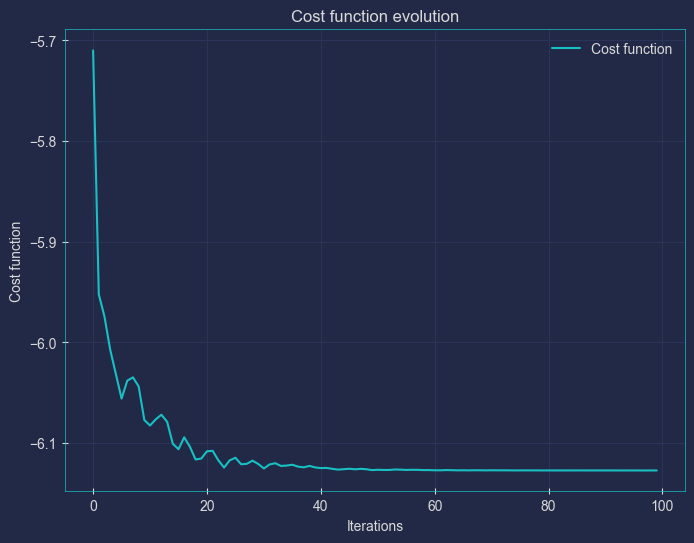
\includegraphics[width=1\textwidth,height=0.75\textwidth]{Figures/Chapter_6/Parity QAOA + Restrictions/Parity+Restriction_Training.png}
        \caption{Plot of the cost function values against the number of iterations during training.}
        \label{fig:Parity+Restriction_Training}
    \end{subfigure}
    \hfill
    \begin{subfigure}[t]{0.495\textwidth}
        \centering
        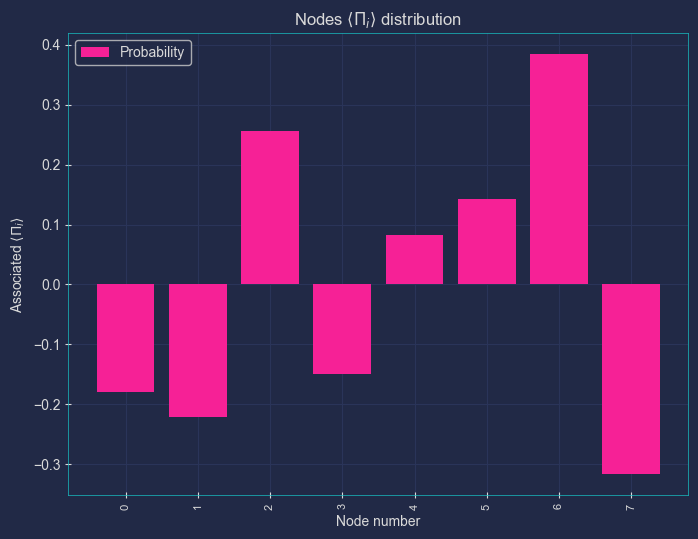
\includegraphics[width=1\textwidth,height=0.75\textwidth]{Figures/Chapter_6/Parity QAOA + Restrictions/Parity+Restriction_Results.png}
        \caption{Plot displaying the expectation values of each node's associated correlator.}
        \label{fig:Parity+Restriction_Results}
    \end{subfigure}
    \caption{Training and results plots for the Parity-like Quantum Approximate Optimization Algorithm (\acrshort{qaoa}), employing enforced regularization to mitigate frustration effects. The partition on the right ($11010001$) corresponds to the \acrshort{maxcut} partition of the usual $8$-node graph ("cut" $ = 10$).}
    \label{fig:Parity+Restriction}
\end{figure*}

%%%%%%%%%%%%%%%%%%%%%%%%%%%%%%%%%%%%%%%%%%%%%%%%%%%%%%%%%%%%%%%%%%%%%%%%
\section{Batch-based Oracle Coloring}
\label{section:Oracle_Coloring}
Another idea we're interested in exploring is the following. Inspired by the previous concept that knowing the correlation between nodes is, trivially, enough to deduce the graph's partition into two colors, we can design a new scheme which makes use of this to compute the \acrshort{maxcut} partition. In short, this scheme could be implemented with a trainable Oracle, which would receive $k < n$ qubits, and return the colors of $k$ nodes. Afterwards, we would run $\frac{n}{k}$ batches of this, to obtain all the $n$ nodes' colors. Algorithmically (Algorithm \ref{alg:BOC}), one could write:

\begin{algorithm}
\caption{Batch-based Oracle coloring (BOC)}\label{alg:BOC}
\begin{algorithmic}
\State Fix a certain value $k < n$ (dimension of batches).
\For{$i = 1$ to $\frac{n}{k}$}
    \State Partition: $\left\{c^i_1, c^i_2, \ldots, c^i_k\right\} \gets O\left(\ket{i}\right)$
    \State $i = i + 1$
\EndFor
\State \textbf{Subroutine:} Utilize the sub-partitions $\left\{c^i_1, c^i_2, \ldots, c^i_k\right\}$ to reconstruct the full graph's partition.
\end{algorithmic}
\end{algorithm}
Although this scheme doesn't explicitly exploit correlations between nodes, a simple variation can be easily formulated in which the Oracle provides the correlation between the inputted nodes.

Returning to Algorithm \ref{alg:BOC}, it's important to ensure that the input state going into the Oracle varies for different values of $i$, allowing the Oracle to distinguish between the batches. However, several nuances need to be addressed in this approach. One crucial consideration is how to train such an Oracle effectively. Training it separately on the sub-graph instances of the original graph may overlook edges connecting different sub-graphs. Thus, a clever approach is needed to incorporate this connectivity during training. 

Another possibility is training multiple Oracles, each dedicated to a specific sub-graph instance. This idea emerged from discussions about what should be provided as input to the scheme. Should it be simply $\ket{i}$ or something like $\ket{i \text{ mod } k}$? The former approach might not utilize all $2^k$ available "entrance" basis states effectively, limiting the encoding of meaningful information to only the first $\frac{n}{k}$ states. Additionally, a constraint arises from the requirement that $2^k$ must be greater than or equal to $\frac{n}{k}$ for the scheme to be valid, which may not hold true for all combinations of $n$ and $k$. This is relevant because we have \( k \) qubits entering and leaving the Oracle. If \( 2^k < \frac{n}{k} \), there aren't enough basis states to encode the total number of required batches, which would be problematic.

These complexities must be carefully considered in the design of the algorithm. However, we have decided to set aside this scheme for now. We found several papers, such as \cite{li2021largescale} and \cite{zhou2022qaoainqaoa}, that address this exact problem, providing numerous solutions with varying degrees of effectiveness. Notably, \cite{zhou2022qaoainqaoa}, titled \textit{"QAOA-in-QAOA: solving large-scale MaxCut problems on small quantum machines"}, particularly captured our attention. It presents insightful approaches that closely align with our original intention of solving \acrshort{maxcut} by addressing sub-graphs individually.
